\documentclass[11pt]{article}

    \usepackage[breakable]{tcolorbox}
    \usepackage{polski}
    \usepackage{parskip} % Stop auto-indenting (to mimic markdown behaviour)
    
    \usepackage{iftex}
    \ifPDFTeX
    	\usepackage[T1]{fontenc}
    	\usepackage{mathpazo}
    \else
    	\usepackage{fontspec}
    \fi

    % Basic figure setup, for now with no caption control since it's done
    % automatically by Pandoc (which extracts ![](path) syntax from Markdown).
    \usepackage{graphicx}
    % Maintain compatibility with old templates. Remove in nbconvert 6.0
    \let\Oldincludegraphics\includegraphics
    % Ensure that by default, figures have no caption (until we provide a
    % proper Figure object with a Caption API and a way to capture that
    % in the conversion process - todo).
    \usepackage{caption}
    \DeclareCaptionFormat{nocaption}{}
    \captionsetup{format=nocaption,aboveskip=0pt,belowskip=0pt}

    \usepackage[Export]{adjustbox} % Used to constrain images to a maximum size
    \adjustboxset{max size={0.9\linewidth}{0.9\paperheight}}
    \usepackage{float}
    \floatplacement{figure}{H} % forces figures to be placed at the correct location
    \usepackage{xcolor} % Allow colors to be defined
    \usepackage{enumerate} % Needed for markdown enumerations to work
    \usepackage{geometry} % Used to adjust the document margins
    \usepackage{amsmath} % Equations
    \usepackage{amssymb} % Equations
    \usepackage{textcomp} % defines textquotesingle
    % Hack from http://tex.stackexchange.com/a/47451/13684:
    \AtBeginDocument{%
        \def\PYZsq{\textquotesingle}% Upright quotes in Pygmentized code
    }
    \usepackage{upquote} % Upright quotes for verbatim code
    \usepackage{eurosym} % defines \euro
    \usepackage[mathletters]{ucs} % Extended unicode (utf-8) support
    \usepackage{fancyvrb} % verbatim replacement that allows latex
    \usepackage{grffile} % extends the file name processing of package graphics 
                         % to support a larger range
    \makeatletter % fix for grffile with XeLaTeX
    \def\Gread@@xetex#1{%
      \IfFileExists{"\Gin@base".bb}%
      {\Gread@eps{\Gin@base.bb}}%
      {\Gread@@xetex@aux#1}%
    }
    \makeatother

    % The hyperref package gives us a pdf with properly built
    % internal navigation ('pdf bookmarks' for the table of contents,
    % internal cross-reference links, web links for URLs, etc.)
    \usepackage{hyperref}
    % The default LaTeX title has an obnoxious amount of whitespace. By default,
    % titling removes some of it. It also provides customization options.
    \usepackage{titling}
    \usepackage{longtable} % longtable support required by pandoc >1.10
    \usepackage{booktabs}  % table support for pandoc > 1.12.2
    \usepackage[inline]{enumitem} % IRkernel/repr support (it uses the enumerate* environment)
    \usepackage[normalem]{ulem} % ulem is needed to support strikethroughs (\sout)
                                % normalem makes italics be italics, not underlines
    \usepackage{mathrsfs}
    
	\author{Piotr Krawiec, Maksymilian Jucha}
    
    % Colors for the hyperref package
    \definecolor{urlcolor}{rgb}{0,.145,.698}
    \definecolor{linkcolor}{rgb}{.71,0.21,0.01}
    \definecolor{citecolor}{rgb}{.12,.54,.11}

    % ANSI colors
    \definecolor{ansi-black}{HTML}{3E424D}
    \definecolor{ansi-black-intense}{HTML}{282C36}
    \definecolor{ansi-red}{HTML}{E75C58}
    \definecolor{ansi-red-intense}{HTML}{B22B31}
    \definecolor{ansi-green}{HTML}{00A250}
    \definecolor{ansi-green-intense}{HTML}{007427}
    \definecolor{ansi-yellow}{HTML}{DDB62B}
    \definecolor{ansi-yellow-intense}{HTML}{B27D12}
    \definecolor{ansi-blue}{HTML}{208FFB}
    \definecolor{ansi-blue-intense}{HTML}{0065CA}
    \definecolor{ansi-magenta}{HTML}{D160C4}
    \definecolor{ansi-magenta-intense}{HTML}{A03196}
    \definecolor{ansi-cyan}{HTML}{60C6C8}
    \definecolor{ansi-cyan-intense}{HTML}{258F8F}
    \definecolor{ansi-white}{HTML}{C5C1B4}
    \definecolor{ansi-white-intense}{HTML}{A1A6B2}
    \definecolor{ansi-default-inverse-fg}{HTML}{FFFFFF}
    \definecolor{ansi-default-inverse-bg}{HTML}{000000}

    % commands and environments needed by pandoc snippets
    % extracted from the output of `pandoc -s`
    \providecommand{\tightlist}{%
      \setlength{\itemsep}{0pt}\setlength{\parskip}{0pt}}
    \DefineVerbatimEnvironment{Highlighting}{Verbatim}{commandchars=\\\{\}}
    % Add ',fontsize=\small' for more characters per line
    \newenvironment{Shaded}{}{}
    \newcommand{\KeywordTok}[1]{\textcolor[rgb]{0.00,0.44,0.13}{\textbf{{#1}}}}
    \newcommand{\DataTypeTok}[1]{\textcolor[rgb]{0.56,0.13,0.00}{{#1}}}
    \newcommand{\DecValTok}[1]{\textcolor[rgb]{0.25,0.63,0.44}{{#1}}}
    \newcommand{\BaseNTok}[1]{\textcolor[rgb]{0.25,0.63,0.44}{{#1}}}
    \newcommand{\FloatTok}[1]{\textcolor[rgb]{0.25,0.63,0.44}{{#1}}}
    \newcommand{\CharTok}[1]{\textcolor[rgb]{0.25,0.44,0.63}{{#1}}}
    \newcommand{\StringTok}[1]{\textcolor[rgb]{0.25,0.44,0.63}{{#1}}}
    \newcommand{\CommentTok}[1]{\textcolor[rgb]{0.38,0.63,0.69}{\textit{{#1}}}}
    \newcommand{\OtherTok}[1]{\textcolor[rgb]{0.00,0.44,0.13}{{#1}}}
    \newcommand{\AlertTok}[1]{\textcolor[rgb]{1.00,0.00,0.00}{\textbf{{#1}}}}
    \newcommand{\FunctionTok}[1]{\textcolor[rgb]{0.02,0.16,0.49}{{#1}}}
    \newcommand{\RegionMarkerTok}[1]{{#1}}
    \newcommand{\ErrorTok}[1]{\textcolor[rgb]{1.00,0.00,0.00}{\textbf{{#1}}}}
    \newcommand{\NormalTok}[1]{{#1}}
    
    % Additional commands for more recent versions of Pandoc
    \newcommand{\ConstantTok}[1]{\textcolor[rgb]{0.53,0.00,0.00}{{#1}}}
    \newcommand{\SpecialCharTok}[1]{\textcolor[rgb]{0.25,0.44,0.63}{{#1}}}
    \newcommand{\VerbatimStringTok}[1]{\textcolor[rgb]{0.25,0.44,0.63}{{#1}}}
    \newcommand{\SpecialStringTok}[1]{\textcolor[rgb]{0.73,0.40,0.53}{{#1}}}
    \newcommand{\ImportTok}[1]{{#1}}
    \newcommand{\DocumentationTok}[1]{\textcolor[rgb]{0.73,0.13,0.13}{\textit{{#1}}}}
    \newcommand{\AnnotationTok}[1]{\textcolor[rgb]{0.38,0.63,0.69}{\textbf{\textit{{#1}}}}}
    \newcommand{\CommentVarTok}[1]{\textcolor[rgb]{0.38,0.63,0.69}{\textbf{\textit{{#1}}}}}
    \newcommand{\VariableTok}[1]{\textcolor[rgb]{0.10,0.09,0.49}{{#1}}}
    \newcommand{\ControlFlowTok}[1]{\textcolor[rgb]{0.00,0.44,0.13}{\textbf{{#1}}}}
    \newcommand{\OperatorTok}[1]{\textcolor[rgb]{0.40,0.40,0.40}{{#1}}}
    \newcommand{\BuiltInTok}[1]{{#1}}
    \newcommand{\ExtensionTok}[1]{{#1}}
    \newcommand{\PreprocessorTok}[1]{\textcolor[rgb]{0.74,0.48,0.00}{{#1}}}
    \newcommand{\AttributeTok}[1]{\textcolor[rgb]{0.49,0.56,0.16}{{#1}}}
    \newcommand{\InformationTok}[1]{\textcolor[rgb]{0.38,0.63,0.69}{\textbf{\textit{{#1}}}}}
    \newcommand{\WarningTok}[1]{\textcolor[rgb]{0.38,0.63,0.69}{\textbf{\textit{{#1}}}}}
    
    
    % Define a nice break command that doesn't care if a line doesn't already
    % exist.
    \def\br{\hspace*{\fill} \\* }
    % Math Jax compatibility definitions
    \def\gt{>}
    \def\lt{<}
    \let\Oldtex\TeX
    \let\Oldlatex\LaTeX
    \renewcommand{\TeX}{\textrm{\Oldtex}}
    \renewcommand{\LaTeX}{\textrm{\Oldlatex}}
    % Document parameters
    % Document title
    \title{Sprawozdanie}
    
    
    
    
    
% Pygments definitions
\makeatletter
\def\PY@reset{\let\PY@it=\relax \let\PY@bf=\relax%
    \let\PY@ul=\relax \let\PY@tc=\relax%
    \let\PY@bc=\relax \let\PY@ff=\relax}
\def\PY@tok#1{\csname PY@tok@#1\endcsname}
\def\PY@toks#1+{\ifx\relax#1\empty\else%
    \PY@tok{#1}\expandafter\PY@toks\fi}
\def\PY@do#1{\PY@bc{\PY@tc{\PY@ul{%
    \PY@it{\PY@bf{\PY@ff{#1}}}}}}}
\def\PY#1#2{\PY@reset\PY@toks#1+\relax+\PY@do{#2}}

\expandafter\def\csname PY@tok@w\endcsname{\def\PY@tc##1{\textcolor[rgb]{0.73,0.73,0.73}{##1}}}
\expandafter\def\csname PY@tok@c\endcsname{\let\PY@it=\textit\def\PY@tc##1{\textcolor[rgb]{0.25,0.50,0.50}{##1}}}
\expandafter\def\csname PY@tok@cp\endcsname{\def\PY@tc##1{\textcolor[rgb]{0.74,0.48,0.00}{##1}}}
\expandafter\def\csname PY@tok@k\endcsname{\let\PY@bf=\textbf\def\PY@tc##1{\textcolor[rgb]{0.00,0.50,0.00}{##1}}}
\expandafter\def\csname PY@tok@kp\endcsname{\def\PY@tc##1{\textcolor[rgb]{0.00,0.50,0.00}{##1}}}
\expandafter\def\csname PY@tok@kt\endcsname{\def\PY@tc##1{\textcolor[rgb]{0.69,0.00,0.25}{##1}}}
\expandafter\def\csname PY@tok@o\endcsname{\def\PY@tc##1{\textcolor[rgb]{0.40,0.40,0.40}{##1}}}
\expandafter\def\csname PY@tok@ow\endcsname{\let\PY@bf=\textbf\def\PY@tc##1{\textcolor[rgb]{0.67,0.13,1.00}{##1}}}
\expandafter\def\csname PY@tok@nb\endcsname{\def\PY@tc##1{\textcolor[rgb]{0.00,0.50,0.00}{##1}}}
\expandafter\def\csname PY@tok@nf\endcsname{\def\PY@tc##1{\textcolor[rgb]{0.00,0.00,1.00}{##1}}}
\expandafter\def\csname PY@tok@nc\endcsname{\let\PY@bf=\textbf\def\PY@tc##1{\textcolor[rgb]{0.00,0.00,1.00}{##1}}}
\expandafter\def\csname PY@tok@nn\endcsname{\let\PY@bf=\textbf\def\PY@tc##1{\textcolor[rgb]{0.00,0.00,1.00}{##1}}}
\expandafter\def\csname PY@tok@ne\endcsname{\let\PY@bf=\textbf\def\PY@tc##1{\textcolor[rgb]{0.82,0.25,0.23}{##1}}}
\expandafter\def\csname PY@tok@nv\endcsname{\def\PY@tc##1{\textcolor[rgb]{0.10,0.09,0.49}{##1}}}
\expandafter\def\csname PY@tok@no\endcsname{\def\PY@tc##1{\textcolor[rgb]{0.53,0.00,0.00}{##1}}}
\expandafter\def\csname PY@tok@nl\endcsname{\def\PY@tc##1{\textcolor[rgb]{0.63,0.63,0.00}{##1}}}
\expandafter\def\csname PY@tok@ni\endcsname{\let\PY@bf=\textbf\def\PY@tc##1{\textcolor[rgb]{0.60,0.60,0.60}{##1}}}
\expandafter\def\csname PY@tok@na\endcsname{\def\PY@tc##1{\textcolor[rgb]{0.49,0.56,0.16}{##1}}}
\expandafter\def\csname PY@tok@nt\endcsname{\let\PY@bf=\textbf\def\PY@tc##1{\textcolor[rgb]{0.00,0.50,0.00}{##1}}}
\expandafter\def\csname PY@tok@nd\endcsname{\def\PY@tc##1{\textcolor[rgb]{0.67,0.13,1.00}{##1}}}
\expandafter\def\csname PY@tok@s\endcsname{\def\PY@tc##1{\textcolor[rgb]{0.73,0.13,0.13}{##1}}}
\expandafter\def\csname PY@tok@sd\endcsname{\let\PY@it=\textit\def\PY@tc##1{\textcolor[rgb]{0.73,0.13,0.13}{##1}}}
\expandafter\def\csname PY@tok@si\endcsname{\let\PY@bf=\textbf\def\PY@tc##1{\textcolor[rgb]{0.73,0.40,0.53}{##1}}}
\expandafter\def\csname PY@tok@se\endcsname{\let\PY@bf=\textbf\def\PY@tc##1{\textcolor[rgb]{0.73,0.40,0.13}{##1}}}
\expandafter\def\csname PY@tok@sr\endcsname{\def\PY@tc##1{\textcolor[rgb]{0.73,0.40,0.53}{##1}}}
\expandafter\def\csname PY@tok@ss\endcsname{\def\PY@tc##1{\textcolor[rgb]{0.10,0.09,0.49}{##1}}}
\expandafter\def\csname PY@tok@sx\endcsname{\def\PY@tc##1{\textcolor[rgb]{0.00,0.50,0.00}{##1}}}
\expandafter\def\csname PY@tok@m\endcsname{\def\PY@tc##1{\textcolor[rgb]{0.40,0.40,0.40}{##1}}}
\expandafter\def\csname PY@tok@gh\endcsname{\let\PY@bf=\textbf\def\PY@tc##1{\textcolor[rgb]{0.00,0.00,0.50}{##1}}}
\expandafter\def\csname PY@tok@gu\endcsname{\let\PY@bf=\textbf\def\PY@tc##1{\textcolor[rgb]{0.50,0.00,0.50}{##1}}}
\expandafter\def\csname PY@tok@gd\endcsname{\def\PY@tc##1{\textcolor[rgb]{0.63,0.00,0.00}{##1}}}
\expandafter\def\csname PY@tok@gi\endcsname{\def\PY@tc##1{\textcolor[rgb]{0.00,0.63,0.00}{##1}}}
\expandafter\def\csname PY@tok@gr\endcsname{\def\PY@tc##1{\textcolor[rgb]{1.00,0.00,0.00}{##1}}}
\expandafter\def\csname PY@tok@ge\endcsname{\let\PY@it=\textit}
\expandafter\def\csname PY@tok@gs\endcsname{\let\PY@bf=\textbf}
\expandafter\def\csname PY@tok@gp\endcsname{\let\PY@bf=\textbf\def\PY@tc##1{\textcolor[rgb]{0.00,0.00,0.50}{##1}}}
\expandafter\def\csname PY@tok@go\endcsname{\def\PY@tc##1{\textcolor[rgb]{0.53,0.53,0.53}{##1}}}
\expandafter\def\csname PY@tok@gt\endcsname{\def\PY@tc##1{\textcolor[rgb]{0.00,0.27,0.87}{##1}}}
\expandafter\def\csname PY@tok@err\endcsname{\def\PY@bc##1{\setlength{\fboxsep}{0pt}\fcolorbox[rgb]{1.00,0.00,0.00}{1,1,1}{\strut ##1}}}
\expandafter\def\csname PY@tok@kc\endcsname{\let\PY@bf=\textbf\def\PY@tc##1{\textcolor[rgb]{0.00,0.50,0.00}{##1}}}
\expandafter\def\csname PY@tok@kd\endcsname{\let\PY@bf=\textbf\def\PY@tc##1{\textcolor[rgb]{0.00,0.50,0.00}{##1}}}
\expandafter\def\csname PY@tok@kn\endcsname{\let\PY@bf=\textbf\def\PY@tc##1{\textcolor[rgb]{0.00,0.50,0.00}{##1}}}
\expandafter\def\csname PY@tok@kr\endcsname{\let\PY@bf=\textbf\def\PY@tc##1{\textcolor[rgb]{0.00,0.50,0.00}{##1}}}
\expandafter\def\csname PY@tok@bp\endcsname{\def\PY@tc##1{\textcolor[rgb]{0.00,0.50,0.00}{##1}}}
\expandafter\def\csname PY@tok@fm\endcsname{\def\PY@tc##1{\textcolor[rgb]{0.00,0.00,1.00}{##1}}}
\expandafter\def\csname PY@tok@vc\endcsname{\def\PY@tc##1{\textcolor[rgb]{0.10,0.09,0.49}{##1}}}
\expandafter\def\csname PY@tok@vg\endcsname{\def\PY@tc##1{\textcolor[rgb]{0.10,0.09,0.49}{##1}}}
\expandafter\def\csname PY@tok@vi\endcsname{\def\PY@tc##1{\textcolor[rgb]{0.10,0.09,0.49}{##1}}}
\expandafter\def\csname PY@tok@vm\endcsname{\def\PY@tc##1{\textcolor[rgb]{0.10,0.09,0.49}{##1}}}
\expandafter\def\csname PY@tok@sa\endcsname{\def\PY@tc##1{\textcolor[rgb]{0.73,0.13,0.13}{##1}}}
\expandafter\def\csname PY@tok@sb\endcsname{\def\PY@tc##1{\textcolor[rgb]{0.73,0.13,0.13}{##1}}}
\expandafter\def\csname PY@tok@sc\endcsname{\def\PY@tc##1{\textcolor[rgb]{0.73,0.13,0.13}{##1}}}
\expandafter\def\csname PY@tok@dl\endcsname{\def\PY@tc##1{\textcolor[rgb]{0.73,0.13,0.13}{##1}}}
\expandafter\def\csname PY@tok@s2\endcsname{\def\PY@tc##1{\textcolor[rgb]{0.73,0.13,0.13}{##1}}}
\expandafter\def\csname PY@tok@sh\endcsname{\def\PY@tc##1{\textcolor[rgb]{0.73,0.13,0.13}{##1}}}
\expandafter\def\csname PY@tok@s1\endcsname{\def\PY@tc##1{\textcolor[rgb]{0.73,0.13,0.13}{##1}}}
\expandafter\def\csname PY@tok@mb\endcsname{\def\PY@tc##1{\textcolor[rgb]{0.40,0.40,0.40}{##1}}}
\expandafter\def\csname PY@tok@mf\endcsname{\def\PY@tc##1{\textcolor[rgb]{0.40,0.40,0.40}{##1}}}
\expandafter\def\csname PY@tok@mh\endcsname{\def\PY@tc##1{\textcolor[rgb]{0.40,0.40,0.40}{##1}}}
\expandafter\def\csname PY@tok@mi\endcsname{\def\PY@tc##1{\textcolor[rgb]{0.40,0.40,0.40}{##1}}}
\expandafter\def\csname PY@tok@il\endcsname{\def\PY@tc##1{\textcolor[rgb]{0.40,0.40,0.40}{##1}}}
\expandafter\def\csname PY@tok@mo\endcsname{\def\PY@tc##1{\textcolor[rgb]{0.40,0.40,0.40}{##1}}}
\expandafter\def\csname PY@tok@ch\endcsname{\let\PY@it=\textit\def\PY@tc##1{\textcolor[rgb]{0.25,0.50,0.50}{##1}}}
\expandafter\def\csname PY@tok@cm\endcsname{\let\PY@it=\textit\def\PY@tc##1{\textcolor[rgb]{0.25,0.50,0.50}{##1}}}
\expandafter\def\csname PY@tok@cpf\endcsname{\let\PY@it=\textit\def\PY@tc##1{\textcolor[rgb]{0.25,0.50,0.50}{##1}}}
\expandafter\def\csname PY@tok@c1\endcsname{\let\PY@it=\textit\def\PY@tc##1{\textcolor[rgb]{0.25,0.50,0.50}{##1}}}
\expandafter\def\csname PY@tok@cs\endcsname{\let\PY@it=\textit\def\PY@tc##1{\textcolor[rgb]{0.25,0.50,0.50}{##1}}}

\def\PYZbs{\char`\\}
\def\PYZus{\char`\_}
\def\PYZob{\char`\{}
\def\PYZcb{\char`\}}
\def\PYZca{\char`\^}
\def\PYZam{\char`\&}
\def\PYZlt{\char`\<}
\def\PYZgt{\char`\>}
\def\PYZsh{\char`\#}
\def\PYZpc{\char`\%}
\def\PYZdl{\char`\$}
\def\PYZhy{\char`\-}
\def\PYZsq{\char`\'}
\def\PYZdq{\char`\"}
\def\PYZti{\char`\~}
% for compatibility with earlier versions
\def\PYZat{@}
\def\PYZlb{[}
\def\PYZrb{]}
\makeatother


    % For linebreaks inside Verbatim environment from package fancyvrb. 
    \makeatletter
        \newbox\Wrappedcontinuationbox 
        \newbox\Wrappedvisiblespacebox 
        \newcommand*\Wrappedvisiblespace {\textcolor{red}{\textvisiblespace}} 
        \newcommand*\Wrappedcontinuationsymbol {\textcolor{red}{\llap{\tiny$\m@th\hookrightarrow$}}} 
        \newcommand*\Wrappedcontinuationindent {3ex } 
        \newcommand*\Wrappedafterbreak {\kern\Wrappedcontinuationindent\copy\Wrappedcontinuationbox} 
        % Take advantage of the already applied Pygments mark-up to insert 
        % potential linebreaks for TeX processing. 
        %        {, <, #, %, $, ' and ": go to next line. 
        %        _, }, ^, &, >, - and ~: stay at end of broken line. 
        % Use of \textquotesingle for straight quote. 
        \newcommand*\Wrappedbreaksatspecials {% 
            \def\PYGZus{\discretionary{\char`\_}{\Wrappedafterbreak}{\char`\_}}% 
            \def\PYGZob{\discretionary{}{\Wrappedafterbreak\char`\{}{\char`\{}}% 
            \def\PYGZcb{\discretionary{\char`\}}{\Wrappedafterbreak}{\char`\}}}% 
            \def\PYGZca{\discretionary{\char`\^}{\Wrappedafterbreak}{\char`\^}}% 
            \def\PYGZam{\discretionary{\char`\&}{\Wrappedafterbreak}{\char`\&}}% 
            \def\PYGZlt{\discretionary{}{\Wrappedafterbreak\char`\<}{\char`\<}}% 
            \def\PYGZgt{\discretionary{\char`\>}{\Wrappedafterbreak}{\char`\>}}% 
            \def\PYGZsh{\discretionary{}{\Wrappedafterbreak\char`\#}{\char`\#}}% 
            \def\PYGZpc{\discretionary{}{\Wrappedafterbreak\char`\%}{\char`\%}}% 
            \def\PYGZdl{\discretionary{}{\Wrappedafterbreak\char`\$}{\char`\$}}% 
            \def\PYGZhy{\discretionary{\char`\-}{\Wrappedafterbreak}{\char`\-}}% 
            \def\PYGZsq{\discretionary{}{\Wrappedafterbreak\textquotesingle}{\textquotesingle}}% 
            \def\PYGZdq{\discretionary{}{\Wrappedafterbreak\char`\"}{\char`\"}}% 
            \def\PYGZti{\discretionary{\char`\~}{\Wrappedafterbreak}{\char`\~}}% 
        } 
        % Some characters . , ; ? ! / are not pygmentized. 
        % This macro makes them "active" and they will insert potential linebreaks 
        \newcommand*\Wrappedbreaksatpunct {% 
            \lccode`\~`\.\lowercase{\def~}{\discretionary{\hbox{\char`\.}}{\Wrappedafterbreak}{\hbox{\char`\.}}}% 
            \lccode`\~`\,\lowercase{\def~}{\discretionary{\hbox{\char`\,}}{\Wrappedafterbreak}{\hbox{\char`\,}}}% 
            \lccode`\~`\;\lowercase{\def~}{\discretionary{\hbox{\char`\;}}{\Wrappedafterbreak}{\hbox{\char`\;}}}% 
            \lccode`\~`\:\lowercase{\def~}{\discretionary{\hbox{\char`\:}}{\Wrappedafterbreak}{\hbox{\char`\:}}}% 
            \lccode`\~`\?\lowercase{\def~}{\discretionary{\hbox{\char`\?}}{\Wrappedafterbreak}{\hbox{\char`\?}}}% 
            \lccode`\~`\!\lowercase{\def~}{\discretionary{\hbox{\char`\!}}{\Wrappedafterbreak}{\hbox{\char`\!}}}% 
            \lccode`\~`\/\lowercase{\def~}{\discretionary{\hbox{\char`\/}}{\Wrappedafterbreak}{\hbox{\char`\/}}}% 
            \catcode`\.\active
            \catcode`\,\active 
            \catcode`\;\active
            \catcode`\:\active
            \catcode`\?\active
            \catcode`\!\active
            \catcode`\/\active 
            \lccode`\~`\~ 	
        }
    \makeatother

    \let\OriginalVerbatim=\Verbatim
    \makeatletter
    \renewcommand{\Verbatim}[1][1]{%
        %\parskip\z@skip
        \sbox\Wrappedcontinuationbox {\Wrappedcontinuationsymbol}%
        \sbox\Wrappedvisiblespacebox {\FV@SetupFont\Wrappedvisiblespace}%
        \def\FancyVerbFormatLine ##1{\hsize\linewidth
            \vtop{\raggedright\hyphenpenalty\z@\exhyphenpenalty\z@
                \doublehyphendemerits\z@\finalhyphendemerits\z@
                \strut ##1\strut}%
        }%
        % If the linebreak is at a space, the latter will be displayed as visible
        % space at end of first line, and a continuation symbol starts next line.
        % Stretch/shrink are however usually zero for typewriter font.
        \def\FV@Space {%
            \nobreak\hskip\z@ plus\fontdimen3\font minus\fontdimen4\font
            \discretionary{\copy\Wrappedvisiblespacebox}{\Wrappedafterbreak}
            {\kern\fontdimen2\font}%
        }%
        
        % Allow breaks at special characters using \PYG... macros.
        \Wrappedbreaksatspecials
        % Breaks at punctuation characters . , ; ? ! and / need catcode=\active 	
        \OriginalVerbatim[#1,codes*=\Wrappedbreaksatpunct]%
    }
    \makeatother

    % Exact colors from NB
    \definecolor{incolor}{HTML}{303F9F}
    \definecolor{outcolor}{HTML}{D84315}
    \definecolor{cellborder}{HTML}{CFCFCF}
    \definecolor{cellbackground}{HTML}{F7F7F7}
    
    % prompt
    \makeatletter
    \newcommand{\boxspacing}{\kern\kvtcb@left@rule\kern\kvtcb@boxsep}
    \makeatother
    \newcommand{\prompt}[4]{
        \ttfamily\llap{{\color{#2}[#3]:\hspace{3pt}#4}}\vspace{-\baselineskip}
    }
    

    
    % Prevent overflowing lines due to hard-to-break entities
    \sloppy 
    % Setup hyperref package
    \hypersetup{
      breaklinks=true,  % so long urls are correctly broken across lines
      colorlinks=true,
      urlcolor=urlcolor,
      linkcolor=linkcolor,
      citecolor=citecolor,
      }
    % Slightly bigger margins than the latex defaults
    
    \geometry{verbose,tmargin=1in,bmargin=1in,lmargin=1in,rmargin=1in}
    
    

\begin{document}
    
    \maketitle
    
    

    
    \hypertarget{sortwanie-szybkie}{%
\section{Sortwanie szybkie}\label{sortwanie-szybkie}}

\hypertarget{opis-algorytmu}{%
\subsection{Opis algorytmu}\label{opis-algorytmu}}

Jest to algorytm sortujący. Sortuje on dane poprzez wybranie pewnej
liczby z tablicy, a następnie przekładanie liczb w tej tablicy tak aby
po lewej stronie znalazły się liczby mniejsze od wybranej a po prawej
większe. Następnie wykonuje tą samą operację dla tablicy po lewej i po
prawej stronie.

\hypertarget{kod}{%
\subsection{Kod}\label{kod}}
    \begin{tcolorbox}[breakable, size=fbox, boxrule=1pt, pad at break*=1mm,colback=cellbackground, colframe=cellborder]
\prompt{In}{incolor}{1}{\boxspacing}
\begin{Verbatim}[commandchars=\\\{\}]
\PY{c+c1}{\PYZsh{} Zwraca indeks taki że, po lewej stronie są wartości mniejsze od niego, a po prawej większe.}
\PY{k}{def} \PY{n+nf}{partition}\PY{p}{(}\PY{n}{tab}\PY{p}{,} \PY{n}{low}\PY{p}{,} \PY{n}{high}\PY{p}{)}\PY{p}{:}
    \PY{c+c1}{\PYZsh{} Wybieram indeks high jako wartość względem której będę porównywał elementy i nazwę ją pivot.}
    \PY{n}{pivot} \PY{o}{=} \PY{n}{tab}\PY{p}{[}\PY{n}{high}\PY{p}{]}
    \PY{c+c1}{\PYZsh{} mid to indeks pivot, za którym będą znajdować się wartości większe od pivot.,}
    \PY{c+c1}{\PYZsh{} na początek ustawiam go na pierwszą wartość.}
    \PY{n}{mid} \PY{o}{=} \PY{n}{low}
    \PY{c+c1}{\PYZsh{} Dla każdego elementu w zakresie low\PYZhy{}high}
    \PY{k}{for} \PY{n}{i} \PY{o+ow}{in} \PY{n+nb}{range}\PY{p}{(}\PY{n}{low}\PY{p}{,} \PY{n}{high}\PY{p}{)}\PY{p}{:}
        \PY{c+c1}{\PYZsh{} Jeżeli wartość w tablicy jest mniejsza od pivot}
        \PY{k}{if} \PY{n}{tab}\PY{p}{[}\PY{n}{i}\PY{p}{]} \PY{o}{\PYZlt{}} \PY{n}{pivot}\PY{p}{:}
            \PY{c+c1}{\PYZsh{} Zamieniam miejscami w tablicy obecną wartość z mid}
            \PY{n}{tab}\PY{p}{[}\PY{n}{i}\PY{p}{]}\PY{p}{,} \PY{n}{tab}\PY{p}{[}\PY{n}{mid}\PY{p}{]} \PY{o}{=} \PY{n}{tab}\PY{p}{[}\PY{n}{mid}\PY{p}{]}\PY{p}{,} \PY{n}{tab}\PY{p}{[}\PY{n}{i}\PY{p}{]}
            \PY{c+c1}{\PYZsh{} zwiększam mid o 1}
            \PY{n}{mid}\PY{o}{+}\PY{o}{=}\PY{l+m+mi}{1}
    \PY{n}{tab}\PY{p}{[}\PY{n}{mid}\PY{p}{]}\PY{p}{,} \PY{n}{tab}\PY{p}{[}\PY{n}{high}\PY{p}{]} \PY{o}{=} \PY{n}{tab}\PY{p}{[}\PY{n}{high}\PY{p}{]}\PY{p}{,} \PY{n}{tab}\PY{p}{[}\PY{n}{mid}\PY{p}{]}
    \PY{k}{return} \PY{n}{mid}
            
    
\PY{k}{def} \PY{n+nf}{quicksort}\PY{p}{(}\PY{n}{tab}\PY{p}{,} \PY{n}{low}\PY{p}{,} \PY{n}{high}\PY{p}{)}\PY{p}{:}
    \PY{k}{if} \PY{n}{low} \PY{o}{\PYZlt{}} \PY{n}{high}\PY{p}{:}
        \PY{c+c1}{\PYZsh{} Poprzekładaj tablicę względem ostatniego elementu}
        \PY{n}{mid} \PY{o}{=} \PY{n}{partition}\PY{p}{(}\PY{n}{tab}\PY{p}{,}\PY{n}{low}\PY{p}{,}\PY{n}{high}\PY{p}{)}
        \PY{c+c1}{\PYZsh{} Przekładaj lewą stronę tablicy}
        \PY{n}{quicksort}\PY{p}{(}\PY{n}{tab}\PY{p}{,}\PY{n}{low}\PY{p}{,}\PY{n}{mid}\PY{o}{\PYZhy{}}\PY{l+m+mi}{1}\PY{p}{)}
        \PY{c+c1}{\PYZsh{} Przekłądaj prawą stronę tablicy}
        \PY{n}{quicksort}\PY{p}{(}\PY{n}{tab}\PY{p}{,}\PY{n}{mid}\PY{o}{+}\PY{l+m+mi}{1}\PY{p}{,}\PY{n}{high}\PY{p}{)}
\end{Verbatim}
\end{tcolorbox}

    \hypertarget{schematy-blokowe}{%
\subsection{Schematy blokowe}\label{schematy-blokowe}}

\hypertarget{funkcja-sortujux105ca}{%
\subsubsection{Funkcja sortująca}\label{funkcja-sortujux105ca}}

\begin{figure}
\centering
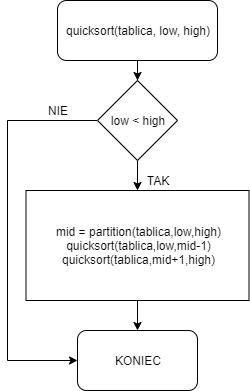
\includegraphics[width=80mm,scale=1.5]{Quicksort/Quicksort.png}
\caption{quicksort}
\end{figure}

\hypertarget{funkcja-przestawiajux105ca-dane-w-tablicy}{%
\subsubsection{Funkcja przestawiająca dane w
tablicy}\label{funkcja-przestawiajux105ca-dane-w-tablicy}}

\begin{figure}
\centering
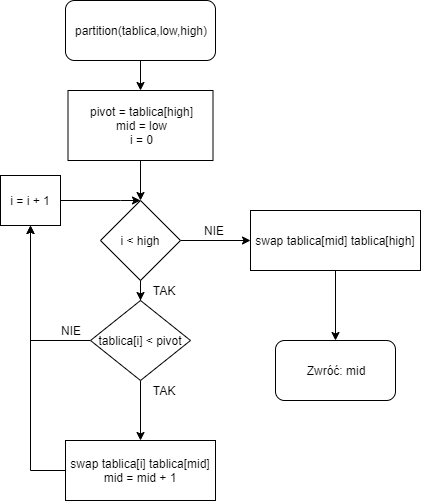
\includegraphics[width=100mm,scale=1.5]{Quicksort/Partition.png}
\caption{quicksort}
\end{figure}

\hypertarget{analiza-matematyczna}{%
\subsection{Analiza}\label{analiza-matematyczna}}

Złożoność tego algorytmu w dużej mierze zależy od tego względem której
liczby będziemy dzielić i przestawiać tablicę. Możemy wyróżnić trzy
przypadki:

\hypertarget{przypadek-pesymistyczny}{%
\subsubsection{Przypadek pesymistyczny}\label{przypadek-pesymistyczny}}

Jako, że zawsze wybieramy ostatnią liczbę algorytm ten będzie dokonywał
największej ilości porównań dla tablicy posortowanej tj. przejdzie po
całej pętli i podzieli ją na dwie tablice, z czego pierwsza będzie
zawierała wszystkie elementy oprócz ostatniego. Zatem wykona się ona $ (n-1) + (n-2) + \ldots{} + 2 + 1 $ razy co daje w sumie 
$ S = \frac{1 + (n-1)}{2} * n = \frac{n^{2}}{2}$

\hypertarget{pozostaux142e-przypadki}{%
\subsubsection{Pozostałe przypadki}\label{pozostaux142e-przypadki}}

W pozostałych przypadkach zakładamy, że trafiamy na liczę która jest w
przybliżeniu medianą liczb sortowanych. Wtedy algorytm dzieli tablicę na
dwie części i osiąga złożoność podobną do sortowania przez scalanie $O(nlog\{n\}) $.

    \hypertarget{doux15bwiadczenia}{%
\subsection{Doświadczenia:}\label{doux15bwiadczenia}}

\hypertarget{doux15bwiadczenie-q1}{%
\subsubsection{Doświadczenie Q1}\label{doux15bwiadczenie-q1}}

\begin{itemize}
\tightlist
\item
  Zakres liczb: -20-20,
\item
  Ilość liczb: 10,
\item
  Sposób wybierania: losowy
\end{itemize}

    \begin{tcolorbox}[breakable, size=fbox, boxrule=1pt, pad at break*=1mm,colback=cellbackground, colframe=cellborder]
\prompt{In}{incolor}{2}{\boxspacing}
\begin{Verbatim}[commandchars=\\\{\}]
\PY{k+kn}{import} \PY{n+nn}{random}
\PY{n}{tablica\PYZus{}przed\PYZus{}posortowaniem} \PY{o}{=} \PY{p}{[}\PY{n}{random}\PY{o}{.}\PY{n}{randrange}\PY{p}{(}\PY{o}{\PYZhy{}}\PY{l+m+mi}{20}\PY{p}{,}\PY{l+m+mi}{21}\PY{p}{)} \PY{k}{for} \PY{n}{i} \PY{o+ow}{in} \PY{n+nb}{range}\PY{p}{(}\PY{l+m+mi}{0}\PY{p}{,}\PY{l+m+mi}{10}\PY{p}{)}\PY{p}{]}

\PY{n+nb}{print}\PY{p}{(}\PY{l+s+s2}{\PYZdq{}}\PY{l+s+s2}{Przed posortowaniem: }\PY{l+s+s2}{\PYZdq{}}\PY{p}{)}
\PY{n+nb}{print}\PY{p}{(}\PY{n}{tablica\PYZus{}przed\PYZus{}posortowaniem}\PY{p}{)}

\PY{n}{posort} \PY{o}{=} \PY{n+nb}{list}\PY{o}{.}\PY{n}{copy}\PY{p}{(}\PY{n}{tablica\PYZus{}przed\PYZus{}posortowaniem}\PY{p}{)}
\PY{n}{quicksort}\PY{p}{(}\PY{n}{posort}\PY{p}{,}\PY{l+m+mi}{0}\PY{p}{,}\PY{n+nb}{len}\PY{p}{(}\PY{n}{posort}\PY{p}{)}\PY{o}{\PYZhy{}}\PY{l+m+mi}{1}\PY{p}{)}

\PY{n+nb}{print}\PY{p}{(}\PY{l+s+s2}{\PYZdq{}}\PY{l+s+s2}{Sortowanie szybkie: }\PY{l+s+s2}{\PYZdq{}}\PY{p}{)}
\PY{n+nb}{print}\PY{p}{(}\PY{n}{posort}\PY{p}{)}
\end{Verbatim}
\end{tcolorbox}

    \begin{Verbatim}[commandchars=\\\{\}]
Przed posortowaniem:
[17, 9, 7, -14, 9, -17, -5, 3, -6, 8]
Sortowanie szybkie:
[-17, -14, -6, -5, 3, 7, 8, 9, 9, 17]
    \end{Verbatim}

    \hypertarget{doux15bwiadczenie-q2}{%
\subsubsection{Doświadczenie Q2}\label{doux15bwiadczenie-q2}}

\begin{itemize}
\tightlist
\item
  Zakres liczb: -1000-1000,
\item
  Ilość liczb: 10 000,
\item
  Sposób wybierania: losowy,
\end{itemize}

    \begin{tcolorbox}[breakable, size=fbox, boxrule=1pt, pad at break*=1mm,colback=cellbackground, colframe=cellborder]
\prompt{In}{incolor}{3}{\boxspacing}
\begin{Verbatim}[commandchars=\\\{\}]
\PY{k+kn}{import} \PY{n+nn}{random}
\PY{k+kn}{from} \PY{n+nn}{timeit} \PY{k}{import} \PY{n}{default\PYZus{}timer} \PY{k}{as} \PY{n}{timer}
\PY{n}{tablica\PYZus{}przed\PYZus{}posortowaniem} \PY{o}{=} \PY{p}{[}\PY{n}{random}\PY{o}{.}\PY{n}{randrange}\PY{p}{(}\PY{o}{\PYZhy{}}\PY{l+m+mi}{1000}\PY{p}{,}\PY{l+m+mi}{1001}\PY{p}{)} \PY{k}{for} \PY{n}{i} \PY{o+ow}{in} \PY{n+nb}{range}\PY{p}{(}\PY{l+m+mi}{0}\PY{p}{,}\PY{l+m+mi}{10000}\PY{p}{)}\PY{p}{]}
\PY{n}{posort} \PY{o}{=} \PY{n+nb}{list}\PY{o}{.}\PY{n}{copy}\PY{p}{(}\PY{n}{tablica\PYZus{}przed\PYZus{}posortowaniem}\PY{p}{)}

\PY{n}{qstart} \PY{o}{=} \PY{n}{timer}\PY{p}{(}\PY{p}{)}
\PY{n}{quicksort}\PY{p}{(}\PY{n}{posort}\PY{p}{,}\PY{l+m+mi}{0}\PY{p}{,}\PY{n+nb}{len}\PY{p}{(}\PY{n}{posort}\PY{p}{)}\PY{o}{\PYZhy{}}\PY{l+m+mi}{1}\PY{p}{)}
\PY{n}{qend} \PY{o}{=} \PY{n}{timer}\PY{p}{(}\PY{p}{)}

\PY{n+nb}{print}\PY{p}{(}\PY{l+s+s2}{\PYZdq{}}\PY{l+s+s2}{Sortowanie szybkie: }\PY{l+s+s2}{\PYZdq{}}\PY{o}{+}\PY{n+nb}{str}\PY{p}{(}\PY{n}{qend} \PY{o}{\PYZhy{}} \PY{n}{qstart}\PY{p}{)}\PY{o}{+} \PY{l+s+s2}{\PYZdq{}}\PY{l+s+s2}{ sekund}\PY{l+s+s2}{\PYZdq{}}\PY{p}{)}
\end{Verbatim}
\end{tcolorbox}

    \begin{Verbatim}[commandchars=\\\{\}]
Sortowanie szybkie: 0.09166770000000013 sekund
    \end{Verbatim}

    \hypertarget{doux15bwiadczenie-q3}{%
\subsubsection{Doświadczenie Q3}\label{doux15bwiadczenie-q3}}

\begin{itemize}
\tightlist
\item
  Zakres licznb: 1-1000,
\item
  Ilość liczb: od 1 do 1000,
\item
  Sposób wybierania: posortowane,
\end{itemize}

    \begin{center}
    \adjustimage{max size={0.9\linewidth}{0.9\paperheight}}{output_8_0.png}
    \end{center}
    { \hspace*{\fill} \\}
    
    \hypertarget{doux15bwiadczenie-q4}{%
\subsubsection{Doświadczenie Q4}\label{doux15bwiadczenie-q4}}

\begin{itemize}
\tightlist
\item
  Zakres licznb: 0-10000,
\item
  Ilość liczb: od 1 do 10000,
\item
  Sposób wybierania: losowe,
\end{itemize}

    \begin{center}
    \adjustimage{max size={0.9\linewidth}{0.9\paperheight}}{output_10_0.png}
    \end{center}
    { \hspace*{\fill} \\}
    
    \hypertarget{doux15bwiadczenie-q5}{%
\subsubsection{Doświadczenie Q5}\label{doux15bwiadczenie-q5}}

\begin{itemize}
\tightlist
\item
  Zakres licznb: 0-10000,
\item
  Ilość liczb: od 1 do 10000,
\item
  Sposób wybierania: prawie posortowane,
\end{itemize}
    \begin{center}
    \adjustimage{max size={0.9\linewidth}{0.9\paperheight}}{output_12_0.png}
    \end{center}
    { \hspace*{\fill} \\}
    
    \hypertarget{wnioski}{%
\subsection{Wnioski}\label{wnioski}}

\begin{itemize}
\tightlist
\item
  Jak widać po doświadczeniu Q3, algorytm ten w tej wersji nie radzi
  sobie dobrze z liczbami które są posortowane, ponieważ zawsze wybiera
  ostatnią liczbę a co za tym idzie, za każdym razem zmiejsza wielkość
  tablicy do posortowania tylko o 1. (Q3)
\item
  Doświadczenia Q1 i Q2 pokazują że algorytm działa i sortuje liczby,
  zarówno ujemne jak i dodatnie. (Q1 i Q2)
\item
  Algorytm bardzo dobrze radzi sobie z dużą liczbą losowych liczb,
  osiągając przy tym złożoność $ O(nlogn) $ (Q4)
\item
  Jak widać dobrze sobie radzie z liczbami które są prawie posortowane
  (Q5)
\end{itemize}

    \hypertarget{sortowanie-bux105belkowe}{%
\section{Sortowanie bąbelkowe}\label{sortowanie-bux105belkowe}}

\hypertarget{opis-algorytmu}{%
\subsection{Opis algorytmu}\label{opis-algorytmu}}

Sortowanie bąbelkowe to algorytm, który przechodzi od początku tablicy
do jej końca porównując kolejne elementy i zamieniając je ze sobą jeżeli
są w złej kolejności. W ten sposób na koniec tablicy trafia zawsze
największa wartość z tej tablicy, dzięku temu kolejne wywołanie
algorytmu przechodzi już tylko do przedostatniego elementu. Cykl ten się
powtarza aż do posortowaniazostanie tylko jeden element.

\hypertarget{kod}{%
\subsection{Kod}\label{kod}}

    \begin{tcolorbox}[breakable, size=fbox, boxrule=1pt, pad at break*=1mm,colback=cellbackground, colframe=cellborder]
\prompt{In}{incolor}{7}{\boxspacing}
\begin{Verbatim}[commandchars=\\\{\}]
\PY{k}{def} \PY{n+nf}{bubbleSort}\PY{p}{(}\PY{n}{sorted\PYZus{}list}\PY{p}{)}\PY{p}{:}
    \PY{k}{for} \PY{n}{nprzejscia} \PY{o+ow}{in} \PY{n+nb}{range}\PY{p}{(}\PY{n+nb}{len}\PY{p}{(}\PY{n}{sorted\PYZus{}list}\PY{p}{)}\PY{o}{\PYZhy{}}\PY{l+m+mi}{1}\PY{p}{,}\PY{l+m+mi}{0}\PY{p}{,}\PY{o}{\PYZhy{}}\PY{l+m+mi}{1}\PY{p}{)}\PY{p}{:}
        \PY{n}{zamiana} \PY{o}{=} \PY{k+kc}{False}
        \PY{k}{for} \PY{n}{i} \PY{o+ow}{in} \PY{n+nb}{range}\PY{p}{(}\PY{n}{nprzejscia}\PY{p}{)}\PY{p}{:}
            \PY{k}{if} \PY{n}{sorted\PYZus{}list}\PY{p}{[}\PY{n}{i}\PY{p}{]}\PY{o}{\PYZgt{}}\PY{n}{sorted\PYZus{}list}\PY{p}{[}\PY{n}{i}\PY{o}{+}\PY{l+m+mi}{1}\PY{p}{]}\PY{p}{:}
                \PY{n}{sorted\PYZus{}list}\PY{p}{[}\PY{n}{i}\PY{p}{]}\PY{p}{,} \PY{n}{sorted\PYZus{}list}\PY{p}{[}\PY{n}{i}\PY{o}{+}\PY{l+m+mi}{1}\PY{p}{]} \PY{o}{=} \PY{n}{sorted\PYZus{}list}\PY{p}{[}\PY{n}{i}\PY{o}{+}\PY{l+m+mi}{1}\PY{p}{]}\PY{p}{,} \PY{n}{sorted\PYZus{}list}\PY{p}{[}\PY{n}{i}\PY{p}{]}
                \PY{n}{zamiana} \PY{o}{=} \PY{k+kc}{True}
        \PY{k}{if} \PY{o+ow}{not} \PY{n}{zamiana}\PY{p}{:}
            \PY{k}{break}
\end{Verbatim}
\end{tcolorbox}

    \hypertarget{schematy-blokowe}{%
\subsection{Schematy blokowe}\label{schematy-blokowe}}

\begin{figure}
\centering
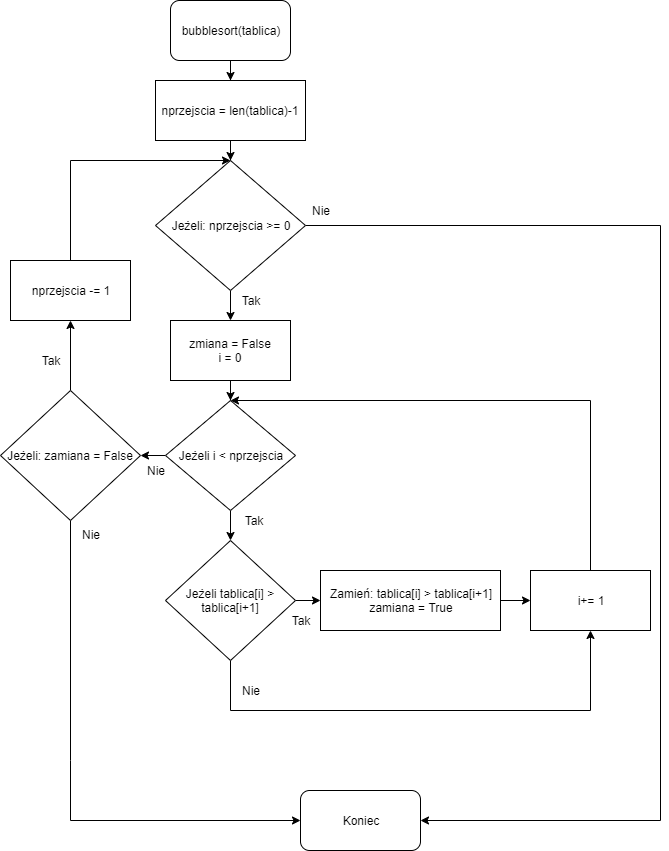
\includegraphics{Bubblesort/Bubble.png}
\caption{quicksort}
\end{figure}

\hypertarget{analiza-matematyczna}{%
\subsection{Analiza}\label{analiza-matematyczna}}

\hypertarget{przypadek-optymistyczny}{%
\subsubsection{Przypadek optymistyczny}\label{przypadek-optymistyczny}}

W tym przypadku algorytm sortuje posortowaną tablicę. Zatem już po
pierwszym przejściu po tablicy z powodu braku zmian zakończy on
działanie osiągają złożoność \(O(n)\).

\hypertarget{pozostaux142e-przypadki}{%
\subsubsection{Pozostałe przypadki}\label{pozostaux142e-przypadki}}

W każdym pozostałym przypadku algorytm ten będzie osiągał złożoność
\(O(n^{2})\)

    

    \hypertarget{doux15bwiadczenia}{%
\subsection{Doświadczenia:}\label{doux15bwiadczenia}}

\hypertarget{doux15bwiadczenie-b1}{%
\subsubsection{Doświadczenie B1}\label{doux15bwiadczenie-b1}}

\begin{itemize}
\tightlist
\item
  Zakres liczb: -20-20,
\item
  Ilość liczb: 10,
\item
  Sposób wybierania: losowy
\end{itemize}

    \begin{tcolorbox}[breakable, size=fbox, boxrule=1pt, pad at break*=1mm,colback=cellbackground, colframe=cellborder]
\prompt{In}{incolor}{8}{\boxspacing}
\begin{Verbatim}[commandchars=\\\{\}]
\PY{k+kn}{import} \PY{n+nn}{random}
\PY{n}{tablica\PYZus{}przed\PYZus{}posortowaniem} \PY{o}{=} \PY{p}{[}\PY{n}{random}\PY{o}{.}\PY{n}{randrange}\PY{p}{(}\PY{o}{\PYZhy{}}\PY{l+m+mi}{20}\PY{p}{,}\PY{l+m+mi}{21}\PY{p}{)} \PY{k}{for} \PY{n}{i} \PY{o+ow}{in} \PY{n+nb}{range}\PY{p}{(}\PY{l+m+mi}{0}\PY{p}{,}\PY{l+m+mi}{10}\PY{p}{)}\PY{p}{]}

\PY{n+nb}{print}\PY{p}{(}\PY{l+s+s2}{\PYZdq{}}\PY{l+s+s2}{Przed posortowaniem: }\PY{l+s+s2}{\PYZdq{}}\PY{p}{)}
\PY{n+nb}{print}\PY{p}{(}\PY{n}{tablica\PYZus{}przed\PYZus{}posortowaniem}\PY{p}{)}

\PY{n}{posort} \PY{o}{=} \PY{n+nb}{list}\PY{o}{.}\PY{n}{copy}\PY{p}{(}\PY{n}{tablica\PYZus{}przed\PYZus{}posortowaniem}\PY{p}{)}
\PY{n}{bubbleSort}\PY{p}{(}\PY{n}{posort}\PY{p}{)}

\PY{n+nb}{print}\PY{p}{(}\PY{l+s+s2}{\PYZdq{}}\PY{l+s+s2}{Sortowanie bąbelkowe: }\PY{l+s+s2}{\PYZdq{}}\PY{p}{)}
\PY{n+nb}{print}\PY{p}{(}\PY{n}{posort}\PY{p}{)}
\end{Verbatim}
\end{tcolorbox}

    \begin{Verbatim}[commandchars=\\\{\}]
Przed posortowaniem:
[6, 6, 20, 18, 2, -10, -15, -2, 10, -19]
Sortowanie bąbelkowe:
[-19, -15, -10, -2, 2, 6, 6, 10, 18, 20]
    \end{Verbatim}

    \hypertarget{doux15bwiadczenie-b2}{%
\subsubsection{Doświadczenie B2}\label{doux15bwiadczenie-b2}}

\begin{itemize}
\tightlist
\item
  Zakres liczb: -1000-1000,
\item
  Ilość liczb: 10 000,
\item
  Sposób wybierania: losowy,
\end{itemize}

    \begin{tcolorbox}[breakable, size=fbox, boxrule=1pt, pad at break*=1mm,colback=cellbackground, colframe=cellborder]
\prompt{In}{incolor}{9}{\boxspacing}
\begin{Verbatim}[commandchars=\\\{\}]
\PY{k+kn}{import} \PY{n+nn}{random}
\PY{k+kn}{from} \PY{n+nn}{timeit} \PY{k}{import} \PY{n}{default\PYZus{}timer} \PY{k}{as} \PY{n}{timer}
\PY{n}{tablica\PYZus{}przed\PYZus{}posortowaniem} \PY{o}{=} \PY{p}{[}\PY{n}{random}\PY{o}{.}\PY{n}{randrange}\PY{p}{(}\PY{o}{\PYZhy{}}\PY{l+m+mi}{1000}\PY{p}{,}\PY{l+m+mi}{1001}\PY{p}{)} \PY{k}{for} \PY{n}{i} \PY{o+ow}{in} \PY{n+nb}{range}\PY{p}{(}\PY{l+m+mi}{0}\PY{p}{,}\PY{l+m+mi}{10000}\PY{p}{)}\PY{p}{]}
\PY{n}{posort} \PY{o}{=} \PY{n+nb}{list}\PY{o}{.}\PY{n}{copy}\PY{p}{(}\PY{n}{tablica\PYZus{}przed\PYZus{}posortowaniem}\PY{p}{)}

\PY{n}{qstart} \PY{o}{=} \PY{n}{timer}\PY{p}{(}\PY{p}{)}
\PY{n}{bubbleSort}\PY{p}{(}\PY{n}{posort}\PY{p}{)}
\PY{n}{qend} \PY{o}{=} \PY{n}{timer}\PY{p}{(}\PY{p}{)}

\PY{n+nb}{print}\PY{p}{(}\PY{l+s+s2}{\PYZdq{}}\PY{l+s+s2}{Sortowanie bąbelkowe: }\PY{l+s+s2}{\PYZdq{}}\PY{o}{+}\PY{n+nb}{str}\PY{p}{(}\PY{n}{qend} \PY{o}{\PYZhy{}} \PY{n}{qstart}\PY{p}{)}\PY{o}{+} \PY{l+s+s2}{\PYZdq{}}\PY{l+s+s2}{ sekund}\PY{l+s+s2}{\PYZdq{}}\PY{p}{)}
\end{Verbatim}
\end{tcolorbox}

    \begin{Verbatim}[commandchars=\\\{\}]
Sortowanie bąbelkowe: 22.224884600000003 sekund
    \end{Verbatim}

    \hypertarget{doux15bwiadczenie-b3}{%
\subsubsection{Doświadczenie B3}\label{doux15bwiadczenie-b3}}

\begin{itemize}
\tightlist
\item
  Zakres licznb: 1-1000,
\item
  Ilość liczb: od 1 do 1000,
\item
  Sposób wybierania: posortowane,
\end{itemize}

    \begin{center}
    \adjustimage{max size={0.9\linewidth}{0.9\paperheight}}{output_23_0.png}
    \end{center}
    { \hspace*{\fill} \\}
    
    \hypertarget{doux15bwiadczenie-b4}{%
\subsubsection{Doświadczenie B4}\label{doux15bwiadczenie-b4}}

\begin{itemize}
\tightlist
\item
  Zakres licznb: 0-10000,
\item
  Ilość liczb: od 1 do 5000,
\item
  Sposób wybierania: losowe,
\end{itemize}


    \begin{center}
    \adjustimage{max size={0.9\linewidth}{0.9\paperheight}}{output_25_0.png}
    \end{center}
    { \hspace*{\fill} \\}
    
    \hypertarget{doux15bwiadczenie-b5}{%
\subsubsection{Doświadczenie B5}\label{doux15bwiadczenie-b5}}

\begin{itemize}
\tightlist
\item
  Zakres licznb: 0-10000,
\item
  Ilość liczb: od 1 do 5000,
\item
  Sposób wybierania: prawie posortowane,
\end{itemize}

    \begin{center}
    \adjustimage{max size={0.9\linewidth}{0.9\paperheight}}{output_27_0.png}
    \end{center}
    { \hspace*{\fill} \\}
    
    \hypertarget{wnioski}{%
\subsection{Wnioski}\label{wnioski}}

\begin{itemize}
\tightlist
\item
  Algorytm dobrze sobie radzi ze sprawdzeniem czy liczby są posortowane
  (B3),
\item
  Algorytm prawidłowo sortuje tablce, zarówno liczby dodatnie jak i
  ujemne (B1 B2),
\item
  Jak widać na doświadczeniu B2 czas sortowania rośnie gwałtownie wraz
  ze wzrostem długości tablicy, wynika to z jego złożoności \(O(n^{2})\)
\item
  Doświadczenia B4 i B5 pokazują, że niezależnie czy liczby są losowe
  czy prawie posortowane algorytm nadal wykona około \(O(n^{2})\)
  iteracji.
\end{itemize}

    \hypertarget{podsumowanie}{%
\section{Podsumowanie}\label{podsumowanie}}

    Jak wynika z powyższych doświadczeń, sortowanie szybkie jest znacznie
bardziej wydajne. Jedyną jego wadą jest to, że zachowuje się jak
bąbelkowe przy posortowanej tablicy, co wynika wyłącznie z tej
implementacji, gdyż wybieram zawsze ostatnią liczbę jako tą względem
której porównuję. W pozostałych przypadkach wyprzedza bąbelkowe, co
szczególnie widać na wykresach Q4 i B4.


    % Add a bibliography block to the postdoc
    
    
    
\end{document}
